\newpage
\section{Introdução à computação clássica.}
Nesse capítulo, você irá aprender os conceitos fundamentais da computação quântica e clássica. Antes de nos aprofundarmos na computação quântica, precisamos de um arcabouço para descrever os qubits e as operações que podemos realizar sobre eles. Para em seguida criar do zero seus primeiros qubits e algoritmos de uma forma prática utilizando NumPy (Numba), PyTorch e Jax. 

 O que você irá aprender:
\begin{itemize}
    \item Entender o que é um Bit e Qubit, como criar, descrever, manipular, representar.
    \item Definir e fornecer exemplos de um sistema quântico em uma superposição e como criar.
    
    \item Declarar a relação entre amplitudes e probabilidades de resultados de medições, e explicar o que significa um estado ser normalizado.
    \item Explicar como operações são aplicadas matematicamente a estados de qubits.
\end{itemize}
 
\newpage
\subsection{A menor unidade de informação: Bit.}
Nesta seção, buscamos responder às seguintes perguntas: 
\begin{center}
    \textit{O que são bits e como os computadores os criam?}
\end{center}
Computadores convencionais, também chamados de computadores clássicos, representam informações por meio de bits. Mas o que é essa informação? Ela pode assumir diversas formas, como imagens, dados de um scanner, impressões digitais, sons ou textos. No entanto, todas essas informações, independentemente de sua natureza, são convertidas em números ou caracteres, que, por sua vez, são transformados em bits. Esses bits consistem em uma sequência de números binários, cada um podendo assumir o valor 0 ou 1. Na tabela a seguir temos 4 exemplos para as letras “a” e "b" e os números $1$ e $2$ : 
\begin{table}[h!]
    \centering
    \begin{tabular}{|c|c|c|}
        \hline
        \textbf{Caractere} & \textbf{Decimal (ASCII)}  & \textbf{Representação em Bits.} \\ \hline
        a & 97 & 01100001 \\ \hline
        b & 98 & 01100010 \\ \hline
        1 & 49 & 00110001 \\ \hline
        2 & 50 & 00110010 \\ \hline
    \end{tabular}
    \caption{Tabela com caracteres e suas representações em valor ASCII (\textit{American Standard Code for Information Interchange}) em binário.}
    \label{tab:caracteres_bits}
\end{table}

O leitor pode estar se perguntando, “como converter caracteres para binário?". 
A conversão de caracteres para binário utilizando a tabela ASCII envolve dois passos principais: identificar o valor decimal correspondente e convertê-lo para binário. Cada caractere possui um código numérico na tabela ASCII, então o primeiro passo é identificar qual o valor decimal do caractere que você quer converter. Por exemplo, a letra \textbf{a} tem valor decimal $97$ e o número $1$ tem valor decimal $49$. O segundo, converter o valor decimal para binário. A conversão para binário pode ser feita dividindo o número decimal sucessivamente por 2, anotando os restos até chegar a zero. Mostraremos isso com exemplos:

\subsubsection*{Exemplo 1: Converter a letra \textbf{a}}
\begin{enumerate}
    \item O código ASCII de \textbf{a} é \textbf{97}.
    \item Dividindo sucessivamente por 2:
    \begin{align*}
        97 \div 2 &= 48 \text{, resto } 1 \\
        48 \div 2 &= 24 \text{, resto } 0 \\
        24 \div 2 &= 12 \text{, resto } 0 \\
        12 \div 2 &= 6 \text{, resto } 0 \\
        6 \div 2 &= 3 \text{, resto } 0 \\
        3 \div 2 &= 1 \text{, resto } 1 \\
        1 \div 2 &= 0 \text{, resto } 1
    \end{align*}
    \item Lendo os restos de baixo para cima: \textbf{01100001}.
\end{enumerate}
Portanto, a letra \textbf{a} em binário é \textbf{01100001}.

\subsubsection*{Exemplo 2: Converter o número \textbf{1}}
\begin{enumerate}
    \item O código ASCII de \textbf{1} é \textbf{49}.
    \item Dividindo sucessivamente por 2:
    \begin{align*}
        49 \div 2 &= 24 \text{, resto } 1 \\
        24 \div 2 &= 12 \text{, resto } 0 \\
        12 \div 2 &= 6 \text{, resto } 0 \\
        6 \div 2 &= 3 \text{, resto } 0 \\
        3 \div 2 &= 1 \text{, resto } 1 \\
        1 \div 2 &= 0 \text{, resto } 1
    \end{align*}
    \item Lendo os restos de baixo para cima: \textbf{00110001}.
\end{enumerate}
Portanto, o número \textbf{1} em binário é \textbf{00110001}\footnote{ Nota: A codificação ASCII utiliza 8 bits para representar cada caractere. Quando o binário resultante possui menos de 8 dígitos, adicionamos zeros à esquerda para completar o padrão. Por isso, o valor \textbf{1100001} torna-se \textbf{01100001}}.

VER ESSA REFERENCIA SOBRE OPERAÇOES CLASSICA DE SOMA MULTIPLICAÇAO COM XOR OR ... :

https://www.makerhero.com/blog/o-que-sao-portas-logicas/?srsltid=AfmBOoodmfMRcMQi3X55XNxUUZQLrTjqgVngCicpLpeuxwAnJp1eJ3mZ
\section*{Exercício Proposto.}
Agora que você aprendeu a converter caracteres para binário, siga os passos descritos no tutorial para realizar as conversões dos seguintes exercícios:

\begin{itemize}
    \item Converta a letra \textbf{b}.
    \item Converta o número \textbf{2}.
\end{itemize}

Para entender como os bits são criados, voltaremos um pouco na história dos computadores. O \textbf{Electronic Numerical Integrator and Computer (ENIAC)} foi um dos primeiros computadores totalmente eletrônicos e digitais de grande escala. Desenvolvido pelos cientistas norte-americanos John Eckert e John Mauchly, o ENIAC começou a operar em fevereiro de 1946. Ele foi projetado para realizar cálculos numéricos complexos, inicialmente voltados para aplicações militares, como o cálculo de trajetórias balísticas. Seu design inovador utilizava cerca de 18.000 válvulas termiônicas (também chamadas de tubos de vácuo), que funcionavam como chaves para representar os estados $0$ e $1$. % Então, para  criar o bit, é sempre necessário associar a algo físico, que pode estar em dois estados diferentes. 

{\color{red} Quantos tempo leva para fazer um cálculo?}

{\color{red} Isso é um tipo de computação analógica?}

{\color{red} Qual o tamanho do dispositivo?}

{\color{red} Qual o tempo para executar um código/protocolo/atividade?}

O ENIAC era programado manualmente por meio da conexão de cabos e da configuração de interruptores. Apesar de sua grande capacidade para a época, era muito trabalhoso reconfigurá-lo para diferentes cálculos, pois isso exigia mudanças físicas nos cabos e chaves. Por outro lado, antes do ENIAC, o \textbf{Mark I}, desenvolvido na Universidade de Harvard, é frequentemente citado como o primeiro computador. No entanto, ele era um dispositivo \textit{eletromecânico}, e não totalmente eletrônico. Isso significa que o Mark I utilizava componentes mecânicos, como relés, combinados com circuitos elétricos para processar dados. Sua operação era consideravelmente mais lenta do que a do ENIAC, devido ao tempo necessário para movimentar as partes mecânicas.

{\color{red} Figura que represente o texto}

Enquanto o Mark I dependia de componentes mecânicos para alternar entre os estados \(0\) e \(1\), o ENIAC representava uma grande evolução ao utilizar válvulas termiônicas, que permitiam transições muito mais rápidas e aumentaram significativamente a velocidade de processamento. Essa mudança marcou o início da era dos computadores eletrônicos. Assim, o ENIAC foi o primeiro computador digital e eletrônico de grande escala, demonstrando o potencial dos sistemas binários na computação e abrindo caminho para o desenvolvimento dos computadores modernos.

Nos computadores modernos, os bits são representados por níveis de tensão elétrica em circuitos integrados. O estado \(0\) representa um nível de tensão mais baixo, que pode ser próximo a \(0\) Volts (V), e o estado \(1\) representa um nível de tensão mais alto, que depende do padrão do circuito. Em processadores modernos da \textbf{AMD} e \textbf{Intel}, a tensão de operação pode variar entre \(0,7\) V a \(1,2\) V para um estado \(1\), enquanto o estado \(0\) é próximo de \(0\) V. A corrente, por sua vez, pode variar dependendo da carga que o circuito está processando, mas, em geral, os processadores modernos operam com correntes muito baixas, na ordem de miliampères (mA), devido ao design eficiente e ao uso de tecnologia de transistores de baixa potência.

Para gerar e controlar os estados binários, os computadores modernos utilizam dispositivos feitos de \textit{semicondutores}, como os \textbf{transistores}. Transistores são dispositivos eletrônicos que funcionam como interruptores, com dois estados possíveis: \textit{ligado} (conduzindo corrente elétrica) e \textit{desligado} (não conduzindo corrente elétrica). Eles são os componentes fundamentais nos circuitos lógicos de qualquer processador. Podemos pensar nos transistores como "nano-interruptores eletrônicos". Eles são extremamente pequenos e rápidos, permitindo a operação de bilhões de transistores em um único chip de computador. Um transistor funciona de maneira semelhante a um interruptor convencional: quando está ligado, permite que a corrente flua, representando o estado $1$; quando está desligado, a corrente não flui, representando o estado $0$.

\begin{figure}
    \centering
    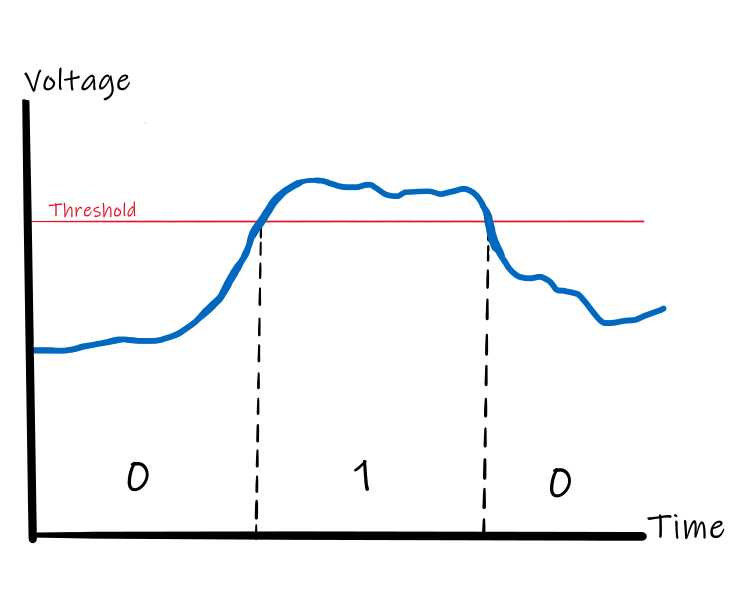
\includegraphics[width=0.5\linewidth]{img/voltage_threshold.png}
    \caption{ Uma tensão elétrica passando por um componente eletrônico usado para representar bits. O threshold é um valor limite para o qual a tensão é associada a um bit no estado 1, e qualquer valor abaixo para um bit no estado 0.}
    \label{fig:enter-label}
\end{figure}

Esses transistores são organizados em \textit{circuitos lógicos} que processam as operações computacionais. Em termos simples, esses circuitos lógicos realizam operações como \textit{E}, \textit{OU}, \textit{NÃO}, combinadas para formar instruções mais complexas. A eficiência e a velocidade dos computadores modernos são na maioria atribuídas ao avanço na miniaturização dos transistores, o que permite que um número maior de operações sejam realizadas por segundo. A velocidade de execução dos computadores modernos é incrivelmente alta devido à miniaturização dos transistores. Processadores atuais, como os da AMD e Intel, podem ter bilhões de transistores em um único chip, com cada transistor ligando e desligando em frações de segundo. A velocidade de comutação dos transistores modernos é da ordem de \textit{gigaherços (GHz)}, ou seja, bilhões de ciclos por segundo.

{\color{red}
Qual o tamanho do dispositivo?}

{\color{red} Qual o tempo para executar um código/protocolo/atividade?}


{\color{red} Qual foi a evolução?}


Comparando com os primeiros computadores, como o ENIAC, a diferença é abismal. O ENIAC tinha componentes como válvulas termiônicas que eram muito mais lentos do que os transistores atuais, além de consumir muito mais energia. Já os transistores modernos, com seu tamanho reduzido para a escala de nanômetros (\(nm\)), operam de forma muito mais eficiente e rápida. Em processadores atuais, o tamanho de um transistor pode ser tão pequeno quanto \(7\) nm, enquanto no ENIAC, os componentes eram muito maiores, e a velocidade de processamento era limitada.


Outro passo importante é como os bits são lidos e interpretados pelos computadores. Para isso, é fundamental compreender o processo de conversão \textit{Analógico-Digital} (A/D). Muitos dispositivos reais, como sensores e microfones, geram sinais \textit{analógicos}, que são contínuos e podem assumir uma infinidade de valores. Por exemplo, um sensor de temperatura pode gerar um valor de tensão que varia continuamente de $0$ a $5$ Volts à medida que a temperatura muda.

No entanto, os computadores trabalham apenas com dados \textit{digitais}, ou seja, dados representados por uma sequência de $0$s e $1$s. Para um sinal analógico ser processado por um computador, ele precisa ser convertido para um formato digital. Isso é feito por dispositivos chamados \textbf{Conversores Analógico-Digital (ADC, do inglês \textit{Analog-to-Digital Converter})}.

Um ADC recebe um sinal analógico e o converte para um valor digital representado por uma sequência de bits. Esse processo ocorre em duas etapas principais:
\begin{enumerate}
    \item \textbf{Amostragem}: O sinal analógico é amostrado em intervalos regulares de tempo. A cada amostra, o valor do sinal analógico é medido.
    \item \textbf{Quantização}: O valor medido da amostra é então arredondado para o valor binário mais próximo, representando a tensão naquele ponto. Quanto maior a resolução do ADC (ou seja, maior o número de bits), mais precisa será a representação do valor analógico.
\end{enumerate}

Por exemplo, se tivermos um sinal analógico variando entre $0$ a $5$ Volts e um ADC de 3 bits, ele poderá representar $8$ valores discretos (de $000$ a $111$) que corresponderiam a diferentes intervalos de tensão. Se o sinal analógico for, por exemplo, $2,5$ Volts, o ADC atribuiria a ele o valor binário $010$, que é o valor mais próximo da tensão medida, na resolução disponível.

Essa conversão analógico-digital permite que dispositivos reais, como sensores de temperatura, pressão, ou até mesmo sinais de áudio, sejam lidos, processados e armazenados pelos computadores, que só conseguem entender valores binários. Assim, a conversão A/D é essencial para integrar o mundo analógico com a computação digital, possibilitando que o computador interaja com o ambiente físico de maneira eficiente.

{\color{red} Problemas e dificuldades da computação clássica. Comentar sobre erros nesses processos}

%Sugestão: Pedir para amandar corrigir a seção bit classico, e adicionar essa parte.



%#####################
\newpage

